\let\negmedspace\undefined
\let\negthickspace\undefined
\documentclass[journal,12pt,onecolumn]{IEEEtran}
\usepackage{cite}
\usepackage{amsmath,amssymb,amsfonts,amsthm}
\usepackage{algorithmic}
\usepackage{graphicx}
\graphicspath{{./figs/}}
\usepackage{textcomp}
\usepackage{xcolor}
\usepackage{txfonts}
\usepackage{listings}
\usepackage{enumitem}
\usepackage{mathtools}
\usepackage{gensymb}
\usepackage{comment}
\usepackage{caption}
\usepackage[breaklinks=true]{hyperref}
\usepackage{tkz-euclide} 
\usepackage{listings}
\usepackage{gvv}                                        
%\def\inputGnumericTable{}                                 
\usepackage[latin1]{inputenc}     
\usepackage{xparse}
\usepackage{color}                                            
\usepackage{array}                                            
\usepackage{longtable}                                       
\usepackage{calc}                                             
\usepackage{multirow}
\usepackage{multicol}
\usepackage{hhline}                                           
\usepackage{ifthen}                                           
\usepackage{lscape}
\usepackage{tabularx}
\usepackage{array}
\usepackage{float}
\newtheorem{theorem}{Theorem}[section]
\newtheorem{problem}{Problem}
\newtheorem{proposition}{Proposition}[section]
\newtheorem{lemma}{Lemma}[section]
\newtheorem{corollary}[theorem]{Corollary}
\newtheorem{example}{Example}[section]
\newtheorem{definition}[problem]{Definition}
\newcommand{\BEQA}{\begin{eqnarray}}
\newcommand{\EEQA}{\end{eqnarray}}
\newcommand{\define}{\stackrel{\triangle}{=}}
\theoremstyle{remark}
\newtheorem{rem}{Remark}


\title{\LARGE \textbf{EE - 2013}}
\author{\Large EE25BTECH11036 - M Chanakya Srinivas}

\date{}
\begin{document}
\maketitle


\begin{enumerate}

\item In the circuit shown below what is the output voltage ($V_{out}$) in Volts if a silicon transistor Q and an ideal op-amp are used?

\begin{center}
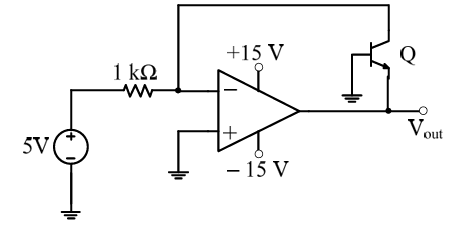
\includegraphics[width=0.5\columnwidth]{figs/1.png}
   \label{fig:placeholder}
\end{center}

\begin{enumerate} 
\begin{multicols}{2}
\item -15  
\item -0.7  
\item +0.7  
\item +15  
 \end{multicols}
 \end{enumerate}

\item The transfer function $\dfrac{V_{2}(s)}{V_{1}(s)}$ of the circuit shown below is

\begin{center}
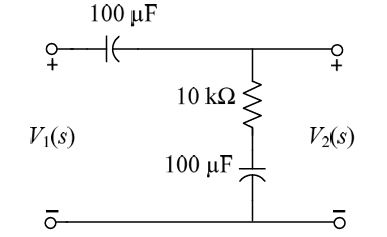
\includegraphics[width=0.5\columnwidth]{figs/2.png} 
   \label{fig:placeholder}
\end{center}

\begin{enumerate} 
\begin{multicols}{2}
\item $\dfrac{0.5s+1}{s+1}$\\
\item $\dfrac{3s+6}{s+2}$  
\item $\dfrac{s+2}{s+2}$\\ 
\item $\dfrac{s+1}{s+2}$  
\end{multicols}
\end{enumerate}

\item Assuming zero initial condition, the response $y(t)$ of the system given below to a unit step input $u(t)$ is

\begin{figure}[h]
    \centering
    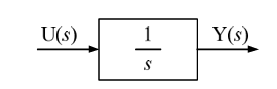
\includegraphics[width=0.5\columnwidth]{figs/3.png}
    \label{fig:placeholder}
\end{figure}

\begin{enumerate}
\begin{multicols}{2}
    
\item $u(t)$ \\
\item $t\,u(t)$  
\item $\dfrac{t^2}{2}u(t)$  \\
\item $e^{t}u(t)$ 
\end{multicols}
\end{enumerate}

\item The impulse response of a system is \begin{align*}
    h(t) = t\,u(t)
\end{align*}
For an input $u(t-1)$, the output is

\begin{enumerate}
\begin{multicols}{2}
    \item $\dfrac{t^2}{2} u(t)$ \\ 
\item $\dfrac{(t-1)u(t-1)}{2}$  
\item $\dfrac{(t-1)^2}{2}u(t-1)$  \\
\item $\dfrac{t^2-1}{2}u(t-1)$
\end{multicols}
\end{enumerate}

\item Which one of the following statements is NOT TRUE for a continuous time causal and stable LTI system?

\begin{enumerate}
\item All the poles of the system must lie on the left side of the $j\omega$ axis.  
\item Zeros of the system can lie anywhere in the $s$-plane.  
\item All the poles must lie within 
\begin{align*}
|s|=1
\end{align*}
\item All the roots of the characteristic equation must be located on the left side of the $j\omega$ axis.  
\end{enumerate}


  \item Two systems with impulse responses $h_1(t)$ and $h_2(t)$ are connected in cascade. Then the overall impulse response of the cascaded system is given by  
  \begin{enumerate}
    \item product of $h_1(t)$ and $h_2(t)$  
    \item sum of $h_1(t)$ and $h_2(t)$  
    \item convolution of $h_1(t)$ and $h_2(t)$  
    \item subtraction of $h_2(t)$ from $h_1(t)$  
  \end{enumerate}

  \item A source 
  \begin{align*}
      v_s(t) = V \cos 1000 t
  \end{align*}
  has an internal impedance of $(4 + j3)\,\ohm$. If a purely resistive load connected to this source has to extract the maximum power out of the source, its value in $\ohm$ should be  
  \begin{enumerate}
  \begin{multicols}{4}
        \item 3 \quad
    \item 4 \quad
    \item 5 \quad
    \item 7  
    \end{multicols}
     \end{enumerate}

  \item A single-phase load is supplied by a single-phase voltage source. If the current flowing from the load to the source is $10\angle -150^\degree \,\text{A}$ and if the voltage at the load terminals is $100\angle 60^\degree\,\text{V}$, then the load  
  \begin{enumerate}
    \item absorbs real power and delivers reactive power  
    \item absorbs real power and absorbs reactive power  
    \item delivers real power and delivers reactive power  
    \item delivers real power and absorbs reactive power  
  \end{enumerate}

  \item A single-phase transformer has a no-load loss of 64 W, as obtained from an open-circuit test. When a short-circuit test is performed on it with 90\% of the rated currents flowing in its both LV and HV windings, the total loss measured is 81 W. The transformer has maximum efficiency when operated at  
  \begin{enumerate}
    \item 50.0\% of the rated current  
    \item 64.0\% of the rated current  
    \item 80.0\% of the rated current  
    \item 88.8\% of the rated current  
  \end{enumerate}

  \item The flux density at a point in space is given by 
  \begin{align*}
      B = 4x a_x + 2k y a_y + 8 a_z  Wb/m^2
  \end{align*}
  The value of constant $k$ must be equal to  
  \begin{enumerate}
  \begin{multicols}{4}
      
 
    \item $-2$ \quad
    \item $-0.5$ \quad
    \item $+0.5$ \quad
    \item $+2$
     \end{multicols}
  \end{enumerate}

  \item A continuous random variable $X$ has a probability density function 
  \begin{align*}
      f(x) = e^{-x}, \; 0 < x < \infty
  \end{align*}
  Then $P[X > 1]$ is  
  \begin{enumerate}
  \begin{multicols}{4}
      
 
    \item 0.368  
    \item 0.5  
    \item 0.632  
    \item 1.0 
     \end{multicols}
  \end{enumerate}

  \item The curl of the gradient of the scalar field defined by 
  \begin{align*}
      V = 2x^2 y + 3y^2 z + 4z^2 x
  \end{align*}is  
  \begin{enumerate}
    \item $4y a_x + 6z a_y + 8x a_z$  
    \item $4a_x + 6a_y + 8a_z$  
    \item $(4xy + 4z^2) a_x + (2x^2 + 6yz) a_y + (3y^2 + 8xz) a_z$  
    \item 0  
  \end{enumerate}

  \item In the feedback network shown below, if the feedback factor $k$ is increased, then the  
  \begin{figure}[h]
      \centering
      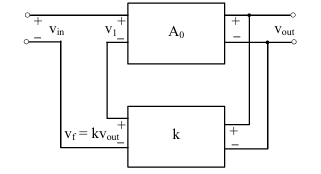
\includegraphics[width=0.5\columnwidth]{figs/4.png}
      \label{fig:placeholder}
  \end{figure}
  \begin{enumerate}
    \item input impedance increases and output impedance decreases  
    \item input impedance increases and output impedance also increases  
    \item input impedance decreases and output impedance also decreases  
    \item input impedance decreases and output impedance increases  
  \end{enumerate}

  \item The input impedance of the permanent magnet moving coil (PMMC) voltmeter is infinite. Assuming that the diode shown in the figure below is ideal, the reading of the voltmeter in Volts is  
\begin{figure}[H]
      \centering
      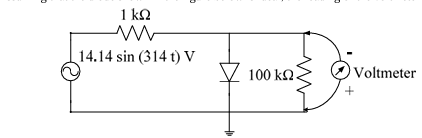
\includegraphics[width=0.5\columnwidth]{figs/5.png}
      \label{fig:placeholder}
  \end{figure}
    \begin{enumerate}
  \begin{multicols}{4}
      

    \item 4.46  
    \item 3.15  
    \item 2.23  
    \item 0
      \end{multicols}
  \end{enumerate}






\item The Bode plot of a transfer function $G(s)$ is shown in the figure below.  

\begin{figure}[H]
    \centering
    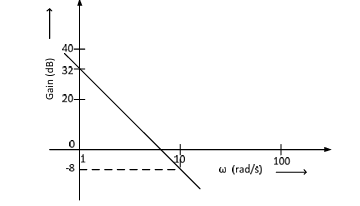
\includegraphics[width=0.5\columnwidth]{figs/6.png}
    \label{fig:placeholder}
\end{figure}
The gain $(20\log|G(j\omega)|)$ is $32$ dB and $-8$ dB at $1$ rad/s and $10$ rad/s respectively. The phase is negative for all $\omega$. Then $G(s)$ is  

\begin{enumerate}
\begin{multicols}{4}
    
\item $\dfrac{39.8}{s}$  
\item $\dfrac{39.8}{s^2}$  
\item $\dfrac{32}{s}$  
\item $\dfrac{32}{s^2}$  
\end{multicols}
\end{enumerate}

\item A bulb in a staircase has two switches, one switch being at the ground floor and the other one at the first floor. The bulb can be turned ON and also can be turned OFF by any one of the switches irrespective of the state of the other switch. The logic of switching of the bulb resembles  

\begin{enumerate}
\begin{multicols}{2}
    
\item An AND gate  
\item An OR gate  
\item An XOR gate  
\item A NAND gate  
\end{multicols}
\end{enumerate}


\item For a periodic signal 
\begin{align*}
    v(t) = 30\sin 100t + 10\cos 300t + 6\sin(500t/\pi),
\end{align*}
the fundamental frequency in rad/s is  

\begin{enumerate}
\begin{multicols}{4}
\item 100  
\item 300  
\item 500  
\item 1500  
\end{multicols}
\end{enumerate}


\item A band-limited signal with a maximum frequency of $5$ kHz is to be sampled. According to the sampling theorem, the sampling frequency in kHz which is NOT valid is  

\begin{enumerate}
\begin{multicols}{4}
    

\item 5  
\item 12  
\item 15  
\item 20  
\end{multicols}
\end{enumerate}


\item Consider a delta connection of resistors and its equivalent star connection as shown below.  
If all elements of the delta connection are scaled by a factor $k, k>0$, the elements of the corresponding star equivalent will be scaled by a factor of  
\begin{figure}[h]
    \centering
    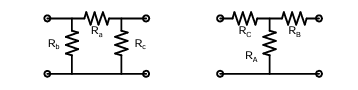
\includegraphics[width=0.5\columnwidth]{figs/7.png}
    \label{fig:placeholder}
\end{figure}
\begin{enumerate}
\begin{multicols}{4}
\item $k^2$  
\item $k$  
\item $1/k$  
\item $\sqrt{k}$
\end{multicols}
\end{enumerate}
\item The angle $\delta$ in the swing equation of a synchronous generator is the  
\begin{enumerate}
\item Angle between stator voltage and current  
\item Angular displacement of the rotor with respect to the stator  
\item Angular displacement of the stator mmf with respect to a synchronously rotating axis  
\item Angular displacement of an axis fixed to the rotor with respect to a synchronously rotating axis  
\end{enumerate}

\item Leakage flux in an induction motor is  
\begin{enumerate}
\item Flux that leaks through the machine  
\item Flux that links both stator and rotor windings  
\item Flux that links the stator winding or the rotor winding but not both  
\item Flux that links the stator winding as well as the rotor winding  
\end{enumerate}

\item In the circuit shown, the type of connections are indicated and shown below.  
Voltmeter readings are $V_1, V_2,$ and $V_3$ as indicated. The correct relation among the voltmeter readings is  


\begin{figure}[h]
    \centering
    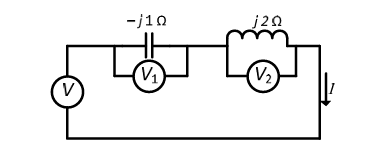
\includegraphics[width=0.5\columnwidth]{figs/8.png}
    \label{fig:placeholder}
\end{figure}
\begin{enumerate}
\begin{multicols}{2}
    
\item $V = \dfrac{V_1}{\sqrt{2}} + \dfrac{V_2}{\sqrt{2}}$  
\item $V = V_1 + V_2$  \\
\item $V = V_1 V_2$  
\item $V = V_1 - V_2$  \\
\end{multicols}
\end{enumerate}

\item Square roots of $-i$, where $i=\sqrt{-1}$, are  
\begin{enumerate}
\item $\pm i$  
\item $\cos\left(\tfrac{-\pi}{4}\right) \pm i\sin\left(\tfrac{-\pi}{4}\right)$  
\item $\cos\left(\tfrac{3\pi}{4}\right) \pm i\sin\left(\tfrac{3\pi}{4}\right)$  
\item $\cos\left(\tfrac{5\pi}{4}\right) \pm i\sin\left(\tfrac{5\pi}{4}\right)$  
\end{enumerate}

\item Given a vector field \begin{align*}
    F = y\hat{i}x - y^2 \hat{a}_x - x^2 \hat{a}_y + x \hat{a}_z
\end{align*}
, the line integral $\int F \cdot dl$ evaluated along a segment on the x-axis from $x=1$ to $x=2$ is  

\begin{enumerate}
\begin{multicols}{4}
    

\item $-2.33$  
\item $0$  
\item $2.33$  
\item $7$  
\end{multicols}
\end{enumerate}

\item The equation 
\[
\myvec{
2 & -2 \\ -1 & 1
}
\myvec{
x_1 \\ x_2
}
=
\myvec{
1 \\ -1
}
\]
has  

\begin{enumerate}
\item No solution  
\item Only one solution  
\item Non-zero unique solution  
\item Multiple solutions  
\end{enumerate}


\section*{Questions Q.26 to Q.31 (2 marks each)}



\item A strain gauge forms one arm of the bridge shown in the figure below and has a nominal resistance without any load as $R_s=300~\ohm$. Other bridge resistances are 
$R_1 = R_2 = R_3 = 300~\ohm$. The maximum permissible current through the strain gauge is $20~\text{mA}$. During certain measurement, when the bridge is excited by maximum permissible voltage and the strain gauge resistance is increased by $1\%$ over the nominal value, the output voltage $V_0$ in mV is
\begin{figure}[h]
    \centering
    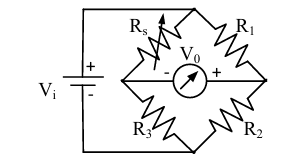
\includegraphics[width=0.5\columnwidth]{figs/9.png}
    \label{fig:placeholder}
\end{figure}
\begin{enumerate}
\begin{multicols}{4}
    

\item 56.02 
\item 40.83
\item 29.85
\item 10.02
\end{multicols}
\end{enumerate}


\item In the circuit shown below, the knee current of the ideal Zener diode is $10~\text{mA}$. To maintain $5~\text{V}$ across $R_L$, the minimum value of $R_1$ in $\ohm$ and the minimum power rating of the Zener diode in mW respectively are
\begin{figure}[h]
    \centering
    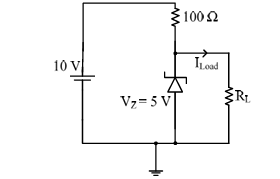
\includegraphics[width=0.5\columnwidth]{figs/10.png}
    \label{fig:placeholder}
\end{figure}
\begin{enumerate}
\begin{multicols}{2}
    

\item 125 and 125
\item 125 and 250
\item 250 and 125
\item 250 and 250
\end{multicols}
\end{enumerate}


\item The open-loop transfer function of a dc motor is given as 
\begin{align*}
    \frac{\omega(s)}{V_a(s)} = \frac{10}{1+10s}.
\end{align*}
When connected in feedback as shown below, the approximate value of $K_a$ that will reduce the time constant of the closed loop system by one hundred times as compared to that of the open-loop system is
\begin{figure}[h]
    \centering
    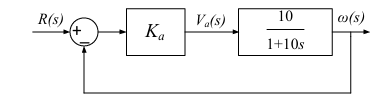
\includegraphics[width=0.5\columnwidth]{figs/11.png}
    \label{fig:placeholder}
\end{figure}
\begin{enumerate}
\begin{multicols}{4}
    

\item 1
\item 5
\item 10
\item 100
\end{multicols}
\end{enumerate}


\item In the circuit shown below, if the source voltage is 
\begin{align*}
    V_s = 100 \angle 53.13^\degree V
\end{align*}
then the Thevenin's equivalent voltage in Volts as seen by the load resistance $R_L$ is
\begin{figure}[h]
    \centering
    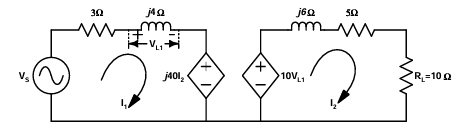
\includegraphics[width=0.5\columnwidth]{figs/12.png}
    \label{fig:placeholder}
\end{figure}
\begin{enumerate}
\begin{multicols}{4}
    

\item $100 \angle 20^\degree$
\item $800 \angle 20^\degree$
\item $800 \angle 290^\degree$
\item $100 \angle 260^\degree$
\end{multicols}
\end{enumerate}


\item Three capacitors $C_1, C_2, C_3$ whose values are $10\mu F, 5\mu F,$ and $2\mu F$ respectively, have breakdown voltages of $10V, 5V,$ and $2V$ respectively. For the interconnection shown, the maximum safe voltage in Volts that can be applied across the combination and the corresponding total charge in $\mu C$ stored in the effective capacitance across the terminals are respectively
\begin{figure}[h]
    \centering
    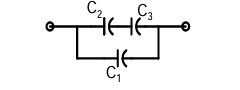
\includegraphics[width=0.5\columnwidth]{figs/13.png}
    \label{fig:placeholder}
\end{figure}
\begin{enumerate}
\begin{multicols}{4}
    

\item 2.8 and 36
\item 7 and 119
\item 2.8 and 32
\item 7 and 80
\end{multicols}
\end{enumerate}


\item A voltage $1000 \sin(\omega t)$ Volts is applied across YZ. Assuming ideal diodes, the voltage measured across WX in Volts is
\begin{figure}[h]
    \centering
    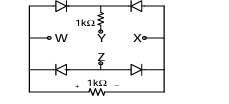
\includegraphics[width=0.5\columnwidth]{figs/14.png}
    \label{fig:placeholder}
\end{figure}
\begin{enumerate}
\begin{multicols}{2}
    

\item $\sin \omega t$\\
\item $\dfrac{\sin \omega t + |\sin \omega t|}{2}$
\item $\dfrac{\sin \omega t - |\sin \omega t|}{2}$\\
\item $0 \;\; \text{for all } t$
\end{multicols}
\end{enumerate}


\item The separately excited dc motor in the figure below has a rated armature current of $20~A$ and a rated armature voltage of $150~V$. An ideal chopper switching at $5~\text{kHz}$ is used to control the armature voltage. If $L_a = 0.1~\text{mH}$, $R_a = 1\ \Omega$, neglecting armature reaction, the duty ratio of the chopper to obtain $50\%$ of the rated torque at the rated speed and the rated field current is
\begin{figure}[h]
    \centering
    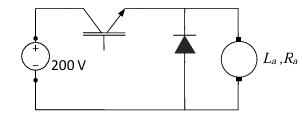
\includegraphics[width=0.5\columnwidth]{figs/15.png}
    \label{fig:placeholder}
\end{figure}
\begin{enumerate}
\begin{multicols}{4}
    \item 0.4
\item 0.5
\item 0.6
\item 0.7
\end{multicols}
\end{enumerate}

\item For a power system network with $n$ nodes, $Z_{ij}$ of its bus impedance matrix is $j0.5$ per unit. The voltage at node $3$ is $1.3 \angle -10^\degree$ per unit. If a capacitor having reactance of $-j3.5$ per unit is now added to the network between node $3$ and the reference node, the current drawn by the capacitor per unit is

\begin{enumerate}
\begin{multicols}{2}
    

\item $0.325 \angle -100^\degree$
\item $0.325 \angle 80^\degree$
\item $0.371 \angle -100^\degree$
\item $0.433 \angle 280^\degree$
\end{multicols}
\end{enumerate}


\item A dielectric slab with $500~\text{mm} \times 500~\text{mm}$ cross-section is $0.4~\text{m}$ long. The slab is subjected to a uniform electric field of 
\begin{align*}
    \mathbf{E} = 6 \mathbf{a_x} + 8 \mathbf{a_y}kV/m
\end{align*}
The relative permittivity of the dielectric material is equal to $2$. The value of constant $\epsilon_0 = 8.854 \times 10^{-12}$ F/m. The energy stored in the dielectric slab in joule is

\begin{enumerate}
\begin{multicols}{4}
    

\item $2.83 \times 10^{-5}$
\item $8.85 \times 10^{-5}$
\item $8.85 \times 10^{-3}$
\item $88.5$
\end{multicols}
\end{enumerate}

\item A matrix has eigenvalues $-1$ and $-2$. The corresponding eigenvectors are 
\[
\myvec{ 1 \\ -1 }, 
\quad
\myvec{ 1 \\ -2 }
\]
respectively. The matrix is

\begin{enumerate}
\begin{multicols}{2}
    

\item \myvec{ 1 & 1 \\ -1 & -2}
\item \myvec{ 1 & 2 \\ -2 & -4 }
\item \myvec{ 0 & -2 \\ -1 & 0 }
\item \myvec{ 0 & 1 \\ -1 & -3 }
\end{multicols}
\end{enumerate}


\item $\displaystyle \int_{|z-i|=2} \frac{z^2-4}{z^2+4} \, dz$ evaluated anticlockwise around the circle $|z-i|=2$, where $i = \sqrt{-1}$, is

\begin{enumerate}
\begin{multicols}{4}

\item $-4\pi i$
\item $0$
\item $2+\pi i$
\item $2+2i$
    
\end{multicols}
\end{enumerate}


\item The clock frequency applied to the digital circuit shown in the figure below is $1~\text{kHz}$. If the initial state of the output Q of the flip-flop is '0', then the frequency of the output waveform Q in kHz is
\begin{figure}[h]
    \centering
    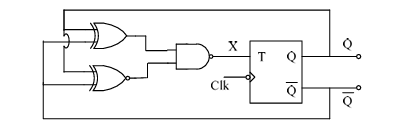
\includegraphics[width=0.5\columnwidth]{figs/16.png}
    \label{fig:placeholder}
\end{figure}
\begin{enumerate}
\begin{multicols}{4}
    

\item 0.25
\item 0.5
\item 1
\item 2
\end{multicols}
\end{enumerate}

\item In the circuit shown below, $Q_1$ has negligible collector-to-emitter saturation voltage and the diode drops negligible voltage across it under forward bias. If 
\begin{align*}
    V_{CE} = +5V
\end{align*}
$X$ and $Y$ are digital signals with $0V$ as logic $0$ and $V_{CE}$ as logic $1$, then the Boolean expression for $Z$ is
\begin{figure}[h]
    \centering
    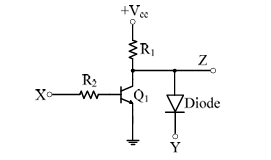
\includegraphics[width=0.5\columnwidth]{figs/17.png}
    \label{fig:placeholder}
\end{figure}
\begin{enumerate}
\begin{multicols}{4}
    

\item $XY$
\item $\overline{X}Y$
\item $X \overline{Y}$
\item $\overline{XY}$
\end{multicols}
\end{enumerate}

\item In the circuit shown below the op-amps are ideal. Then $V_{out}$ in Volts is
\begin{figure}[h]
    \centering
    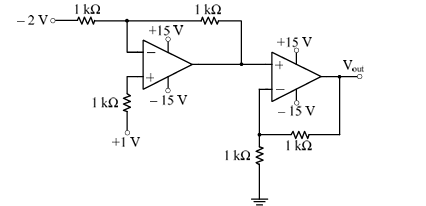
\includegraphics[width=0.5\columnwidth]{figs/18.png}
    \label{fig:placeholder}
\end{figure}
\begin{enumerate}
\begin{multicols}{4}
    

\item 4
\item 6
\item 8
\item 10
\end{multicols}
\end{enumerate}


\section*{Questions Q.40 to Q.49 (2 marks each)}




\item The signal flow graph for a system is given below. The transfer function $\dfrac{Y(s)}{U(s)}$ for this system is
\begin{figure}[h]
    \centering
    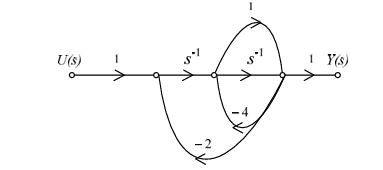
\includegraphics[width=0.5\columnwidth]{figs/19.png}
    \label{fig:placeholder}
\end{figure}
\begin{enumerate}
\begin{multicols}{2}

\item $\dfrac{s+1}{s^3+6s+2}$ \\
\item $\dfrac{s+1}{s^3+6s+2}$
\item $\dfrac{s+1}{s^3+4s+2}$ \\
\item $\dfrac{s+1}{s^3+6s+2}$
    
\end{multicols}
\end{enumerate}


\item The impulse response of a continuous-time system is given by 
\begin{align*}
    h(t) = \delta(t-1)+\delta(t-3)
\end{align*}
The value of the step response at $t=2$ is

\begin{enumerate}
\begin{multicols}{4}
    

\item 0
\item 1
\item 2
\item 3
\end{multicols}
\end{enumerate}

\item Two magnetically uncoupled inductive coils have $Q$ factors $q_1$ and $q_2$ at the chosen operating frequency. Their respective resistances are $R_1$ and $R_2$. When connected in series, their effective $Q$ factor at the same operating frequency is

\begin{enumerate}
\begin{multicols}{2}
    

\item $\dfrac{q_1 R_1 + q_2 R_2}{R_1 + R_2}$\\
\item $\dfrac{q_1 R_2 + q_2 R_1}{R_1 + R_2}$
\item $(q_1 R_1 + q_2 R_2)/(R_1+R_2)$\\
\item $q_1 R_2 + q_2 R_1$
\end{multicols}
\end{enumerate}

\item The following arrangement consists of an ideal transformer and an attenuator which attenuates by a factor of $0.8$. An ac voltage $V_{WX1} = 100V$ is applied across WX to get an open circuit voltage $V_{YZ1}$ across YZ. Next, an ac voltage $V_{YZ2} = 100V$ is applied across YZ to get an open circuit voltage $V_{WX2}$ across WX. Then, $V_{YZ1}, V_{WX1}, V_{WX2}, V_{YZ2}$ are respectively
\begin{figure}[h]
    \centering
    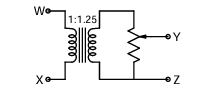
\includegraphics[width=0.5\columnwidth]{figs/20.png}
    \label{fig:placeholder}
\end{figure}
\begin{enumerate}
\begin{multicols}{2}
    

\item 125/100 and 80/100
\item 100/100 and 80/100
\item 100/100 and 100/100
\item 80/100 and 80/100
\end{multicols}
\end{enumerate}


\item Thyristor T in the figure below is initially off and is triggered with a single pulse of width $10\ \mu s$. It is given that $L = \tfrac{(20)}{\pi}\ \mu H$ and $C = \tfrac{(20)}{\pi}\ \mu F$. Assuming latching and holding currents of the thyristor are both zero and the initial charge on C is zero, T conducts for
\begin{figure}[h!]
    \centering
    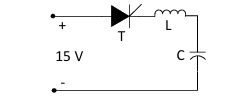
\includegraphics[width=0.5\columnwidth]{figs/21.png}
    \label{fig:placeholder}
\end{figure}
\begin{enumerate}
\begin{multicols}{4}
    

\item $10\ \mu s$
\item $50\ \mu s$
\item $100\ \mu s$
\item $200\ \mu s$
\end{multicols}
\end{enumerate}


\item A 4-pole induction motor, supplied by a slightly unbalanced three-phase $50\ \text{Hz}$ source, is rotating at 1440 rpm. The electrical frequency in Hz of the induced negative sequence current in the rotor is

\begin{enumerate}
\begin{multicols}{4}
    

\item 100
\item 98
\item 52
\item 48
\end{multicols}
\end{enumerate}


\item A function 
\begin{align*}
    y = 5x^2 + 10x
\end{align*}
is defined over an open interval $x=(1,2)$. At least at one point in this interval, $\dfrac{dy}{dx}$ is exactly

\begin{enumerate}
\begin{multicols}{4}
    

\item 20
\item 25
\item 30
\item 35
\end{multicols}
\end{enumerate}


\item When the Newton-Raphson method is applied to solve the equation \begin{align*}
    f(x) = x^2 + 2x - 1 = 0
\end{align*}
the solution at the end of the first iteration with the initial guess value as $x_0 = 1.2$ is

\begin{enumerate}
\begin{multicols}{4}
    

\item $-0.82$
\item $0.49$
\item $0.705$
\item $1.69$
\end{multicols}
\end{enumerate}

\item In the figure shown below, the chopper feeds a resistive load from a battery source. MOSFET Q is switched at 250 kHz, with a duty ratio of 0.4. All elements of the circuit are assumed to be ideal. 
\begin{figure}[H]
    \centering
    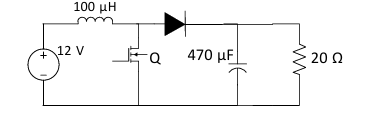
\includegraphics[width=0.5\columnwidth]{figs/22.png}
    \label{fig:placeholder}
\end{figure}
The average source current in Amps in steady-state is

\begin{enumerate}
\begin{multicols}{4}
    

\item 3/2
\item 5/3
\item 5/2
\item 15/4
\end{multicols}
\end{enumerate}


\item The PEAK-TO-PEAK source current ripple in Amps is

\begin{enumerate}
\begin{multicols}{4}
    

\item 0.96
\item 0.144
\item 0.192
\item 0.288
\end{multicols}
\end{enumerate}



\textbf{Common Data for Questions 50 and 51:}

The state variable formulation of a system is given as
\[
\myvec{ 
\dot{x}_1 \\ 
\dot{x}_2 \\ 
\dot{x}_3 
}
=
\myvec{ 
-2 & -2 & 0 \\ 
1 & -1 & 0 \\ 
0 & -1 & -1 
}
\myvec{ 
x_1 \\ 
x_2 \\ 
x_3 
}
+
\myvec{ 
1 \\ 
1 \\ 
1 
}u, 
\quad 
x_1(0)=0, \; x_2(0)=0, \; x_3(0)=0,
\quad
y = [1\;0\;0]
\myvec{ 
x_1 \\ x_2 \\ x_3
}.
\]


\item The system is
\begin{enumerate}

\item controllable but not observable
\item not controllable but observable
\item both controllable and observable
\item both not controllable and not observable
\end{enumerate}

\item The response $y(t)$ to a unit step input is
\begin{enumerate}
\begin{multicols}{2}
    \item $\dfrac{1}{2} - \dfrac{1}{2}e^{-2t}$\\
\item $1 - \dfrac{1}{2}e^{-t} - \dfrac{1}{2}e^{-2t}$
\item $e^{-2t} - e^{-t}$\\
\item $1 - e^{-t}$
\end{multicols}
\end{enumerate}


\textbf{Linked Answer Questions 52 and 53:}

 In the following network, the voltage magnitudes at all buses are equal to 1 p.u., the voltage phase angles are very small, and the line resistances are negligible. All the line reactances are equal to $j1\,\ohm$.

\begin{figure}[H]
    \centering
    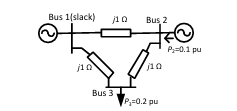
\includegraphics[width=0.5\columnwidth]{figs/23.png}
    \label{fig:placeholder}
\end{figure}

\item The voltage phase angles in rad at buses 2 and 3 are
\begin{enumerate}
\begin{multicols}{2}
    

\item $\theta_2 = -0.1, \;\theta_3 = -0.2$
\item $\theta_2 = 0, \;\theta_3 = -0.1$
\item $\theta_2 = 0.1, \;\theta_3 = 0.1$
\item $\theta_2 = 0.1, \;\theta_3 = 0.2$
\end{multicols}
\end{enumerate}

\item If the base impedance and the line-to-line base voltage are $100 \,\ohm$ and $100 \,\text{kV}$ respectively, then the real power in MW delivered by the generator connected at the slack bus is
\begin{enumerate}
\begin{multicols}{4}
    

\item $-10$
\item $0$
\item $10$
\item $20$
\end{multicols}
\end{enumerate}


\textbf{Statement for Linked Answer Questions 54 and 55:}

The Voltage Source Inverter (VSI) shown in the figure below is switched to provide a $50\,\text{Hz}$ square-wave AC output voltage $(v_o)$ across an $R$,$L$ load Reference polarity of $v_o$ and reference direction of the output current $i_o$ are indicated in the figure. It is given that $R = 3\,\ohm, \; L = 9.55\,\text{mH}$.
\begin{figure}[h]
    \centering
    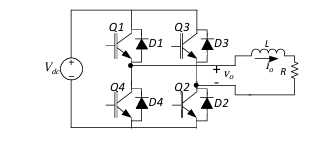
\includegraphics[width=0.5\columnwidth]{figs/24.png}
    \label{fig:placeholder}
\end{figure}



\item In the interval when $v_o < 0$ and $i_o > 0$, the pair of devices which conducts the load current is
\begin{enumerate}
\begin{multicols}{4}

\item Q1, Q2
\item Q3, Q4
\item D1, D2
\item D3, D4
    
\end{multicols}
\end{enumerate}

\item Appropriate transition i.e., Zero Voltage Switching (ZVS)/Zero Current Switching (ZCS) of the IGBTs of the inverter during turn-on/turn-off is
\begin{enumerate}

\item ZVS during turn-off
\item ZVS during turn-on
\item ZCS during turn-off
\item ZCS during turn-on
\end{enumerate}



\section*{General Aptitude (GA) Questions}

\subsection*{Q.56 to Q.60 carry one mark each.}

\item They were requested not to quarrel with others.\\
Which one of the following options is the closest in meaning to the word quarrel?
\begin{enumerate}
\begin{multicols}{4}
    

\item make out
\item call out
\item dig out
\item fall out
\end{multicols}
\end{enumerate}

\item In the summer of 2012, in New Delhi, the mean temperature of Monday to Wednesday was
$41^{\degree}\text{C}$ and of Tuesday to Thursday was $43^{\degree}\text{C}$. If the temperature on Thursday
was $15\%$ higher than that of Monday, then the temperature in $^{\degree}\text{C}$ on Thursday was
\begin{enumerate}
\begin{multicols}{4}
    

\item 40
\item 43
\item 46
\item 49
\end{multicols}
\end{enumerate}

\item Complete the sentence:\\
\emph{Dare \underline{\phantom{to commit}} mistakes.}
\begin{enumerate}
\begin{multicols}{4}
    

\item commit
\item to commit
\item committed
\item committing
\end{multicols}
\end{enumerate}

\item Choose the grammatically \textbf{CORRECT} sentence:
\begin{enumerate}
\item Two and two add four.
\item Two and two become four.
\item Two and two are four.
\item Two and two make four.
\end{enumerate}

\item \textbf{Statement:} You can always give me a ring whenever you need.\\
Which one of the following is the best inference from the above statement?
\begin{enumerate}
\item Because I have a nice caller tune.
\item Because I have a better telephone facility.
\item Because a friend in need is a friend indeed.
\item Because you need not pay towards the telephone bills when you give me a ring.
\end{enumerate}


\subsection*{Q.61 to Q.65 carry two marks each.}


\item What is the chance that a leap year, selected at random, will contain 53 Saturdays?
\begin{enumerate}
\begin{multicols}{4}
    

\item $\dfrac{2}{7}$
\item $\dfrac{3}{7}$
\item $\dfrac{1}{7}$
\item $\dfrac{5}{7}$
\end{multicols}
\end{enumerate}

\item \textbf{Statement:} There were different streams of freedom movements in colonial India carried out by the moderates, liberals, radicals, socialists, and so on.\\
Which one of the following is the best inference from the above statement?
\begin{enumerate}
\item The emergence of nationalism in colonial India led to our Independence.
\item Nationalism in India emerged in the context of colonialism.
\item Nationalism in India is homogeneous.
\item Nationalism in India is heterogeneous.
\end{enumerate}

\item The set of values of $p$ for which the roots of the equation
\begin{align*}
    3x^{2} + 2x + p(p-1) = 0
\end{align*}
are of opposite sign is
\begin{enumerate}
\begin{multicols}{4}

\item $(-\infty,\,0)$
\item $(0,\,1)$
\item $(1,\,\infty)$
\item $(0,\,\infty)$
    
\end{multicols}
\end{enumerate}

\item A car travels $8$ km in the first quarter of an hour, $6$ km in the second quarter and $16$ km in the third quarter. The average speed of the car in km per hour over the entire journey is
\begin{enumerate}
\begin{multicols}{4}
    

\item 30
\item 36
\item 40
\item 24
\end{multicols}
\end{enumerate}

\item Find the sum to $n$ terms of the series $10 + 84 + 734 + \ldots$
\begin{enumerate}
\begin{multicols}{2}
    

\item $\displaystyle\frac{9(9^{n}+1)}{10}+1$\\
\item $\displaystyle \frac{9(9^{n}-1)}{8}+1$
\item $\displaystyle \frac{9(9^{n}-1)}{8}+n$\\
\item $\displaystyle \frac{9(9^{n}-1)}{8}+n^{2}$

\end{multicols}
\end{enumerate}
\end{enumerate}



\end{document}














